\documentclass[10pt,twocolumn]{article}
\usepackage[letterpaper,margin=0.75in,columnsep=0.28in]{geometry}
\usepackage{mathptmx}
\usepackage[T1]{fontenc}
\usepackage{amsmath,amssymb}
\usepackage{booktabs,multirow}
\usepackage{graphicx}
\usepackage{xcolor}
\usepackage{microtype}
\usepackage{enumitem}
\usepackage[font=small,labelfont=bf,skip=4pt]{caption}
\usepackage[numbers,sort&compress]{natbib}
\usepackage{tikz}
\usetikzlibrary{arrows.meta,decorations.pathreplacing,positioning}
\usepackage[colorlinks=true,linkcolor=blue!50!black,citecolor=blue!50!black,urlcolor=blue!50!black]{hyperref}
\usepackage[capitalise,noabbrev]{cleveref}
\setlist{itemsep=1pt,topsep=2pt,leftmargin=12pt}
\setlength{\textfloatsep}{8pt plus 2pt minus 2pt}
\setlength{\dbltextfloatsep}{8pt plus 2pt minus 2pt}
% auto-generated by scripts/make_figures.py -- do not edit
\makeatletter
\newcommand{\AUC}[1]{\@nameuse{auc@#1}}
\newcommand{\AUCsd}[1]{\@nameuse{aucsd@#1}}
\newcommand{\AUPRC}[1]{\@nameuse{auprc@#1}}
\newcommand{\NT}[1]{\@nameuse{nt@#1}}
\newcommand{\RFIVE}[1]{\@nameuse{rfive@#1}}
\newcommand{\RONE}[1]{\@nameuse{rone@#1}}
\newcommand{\RTEN}[1]{\@nameuse{rten@#1}}
\newcommand{\PC}[2]{\@nameuse{pc@#1@#2}}
\newcommand{\SIG}[2]{\@nameuse{sig@#1@#2}}
\newcommand{\MIX}[1]{\@nameuse{mix@#1}}
\newcommand{\CL}[1]{\@nameuse{cl@#1}}
\@namedef{auc@irene_k2}{0.785}\@namedef{aucsd@irene_k2}{0.002}\@namedef{auprc@irene_k2}{0.369}
\@namedef{nt@irene_k2}{0.588}
\@namedef{pc@irene_k2@0}{0.87}
\@namedef{pc@irene_k2@1}{0.77}
\@namedef{pc@irene_k2@2}{0.76}
\@namedef{pc@irene_k2@3}{0.86}
\@namedef{pc@irene_k2@4}{0.82}
\@namedef{pc@irene_k2@5}{0.71}
\@namedef{pc@irene_k2@6}{0.70}
\@namedef{mix@irene_k2}{0.723}
\@namedef{auc@irene_k1}{0.780}\@namedef{aucsd@irene_k1}{0.006}\@namedef{auprc@irene_k1}{0.352}
\@namedef{nt@irene_k1}{0.566}
\@namedef{pc@irene_k1@0}{0.86}
\@namedef{pc@irene_k1@1}{0.70}
\@namedef{pc@irene_k1@2}{0.77}
\@namedef{pc@irene_k1@3}{0.86}
\@namedef{pc@irene_k1@4}{0.85}
\@namedef{pc@irene_k1@5}{0.69}
\@namedef{pc@irene_k1@6}{0.73}
\@namedef{mix@irene_k1}{0.717}
\@namedef{auc@irene_k2_rawtext}{0.794}\@namedef{aucsd@irene_k2_rawtext}{0.008}\@namedef{auprc@irene_k2_rawtext}{0.387}
\@namedef{nt@irene_k2_rawtext}{0.587}
\@namedef{pc@irene_k2_rawtext@0}{0.88}
\@namedef{pc@irene_k2_rawtext@1}{0.73}
\@namedef{pc@irene_k2_rawtext@2}{0.80}
\@namedef{pc@irene_k2_rawtext@3}{0.90}
\@namedef{pc@irene_k2_rawtext@4}{0.83}
\@namedef{pc@irene_k2_rawtext@5}{0.72}
\@namedef{pc@irene_k2_rawtext@6}{0.69}
\@namedef{mix@irene_k2_rawtext}{0.724}
\@namedef{auc@late_clip_l0.5}{0.793}\@namedef{aucsd@late_clip_l0.5}{0.004}\@namedef{auprc@late_clip_l0.5}{0.322}
\@namedef{nt@late_clip_l0.5}{0.699}
\@namedef{rfive@late_clip_l0.5}{13.1}\@namedef{rone@late_clip_l0.5}{3.1}\@namedef{rten@late_clip_l0.5}{21.4}
\@namedef{pc@late_clip_l0.5@0}{0.86}
\@namedef{pc@late_clip_l0.5@1}{0.71}
\@namedef{pc@late_clip_l0.5@2}{0.73}
\@namedef{pc@late_clip_l0.5@3}{0.87}
\@namedef{pc@late_clip_l0.5@4}{0.81}
\@namedef{pc@late_clip_l0.5@5}{0.81}
\@namedef{pc@late_clip_l0.5@6}{0.75}
\@namedef{mix@late_clip_l0.5}{0.720}
\@namedef{auc@irene_k2_nodoc}{0.738}\@namedef{aucsd@irene_k2_nodoc}{0.013}\@namedef{auprc@irene_k2_nodoc}{0.299}
\@namedef{nt@irene_k2_nodoc}{0.599}
\@namedef{pc@irene_k2_nodoc@0}{0.79}
\@namedef{pc@irene_k2_nodoc@1}{0.72}
\@namedef{pc@irene_k2_nodoc@2}{0.62}
\@namedef{pc@irene_k2_nodoc@3}{0.85}
\@namedef{pc@irene_k2_nodoc@4}{0.80}
\@namedef{pc@irene_k2_nodoc@5}{0.65}
\@namedef{pc@irene_k2_nodoc@6}{0.73}
\@namedef{mix@irene_k2_nodoc}{0.701}
\@namedef{auc@attn_bi_cross}{0.752}\@namedef{aucsd@attn_bi_cross}{0.005}\@namedef{auprc@attn_bi_cross}{0.324}
\@namedef{nt@attn_bi_cross}{0.591}
\@namedef{pc@attn_bi_cross@0}{0.85}
\@namedef{pc@attn_bi_cross@1}{0.70}
\@namedef{pc@attn_bi_cross@2}{0.68}
\@namedef{pc@attn_bi_cross@3}{0.86}
\@namedef{pc@attn_bi_cross@4}{0.79}
\@namedef{pc@attn_bi_cross@5}{0.66}
\@namedef{pc@attn_bi_cross@6}{0.72}
\@namedef{mix@attn_bi_cross}{0.692}
\@namedef{auc@late_fusion}{0.794}\@namedef{aucsd@late_fusion}{0.010}\@namedef{auprc@late_fusion}{0.399}
\@namedef{nt@late_fusion}{0.655}
\@namedef{pc@late_fusion@0}{0.88}
\@namedef{pc@late_fusion@1}{0.78}
\@namedef{pc@late_fusion@2}{0.81}
\@namedef{pc@late_fusion@3}{0.84}
\@namedef{pc@late_fusion@4}{0.83}
\@namedef{pc@late_fusion@5}{0.73}
\@namedef{pc@late_fusion@6}{0.69}
\@namedef{mix@late_fusion}{0.729}
\@namedef{auc@clip_l0.1}{0.739}\@namedef{aucsd@clip_l0.1}{0.004}\@namedef{auprc@clip_l0.1}{0.297}
\@namedef{nt@clip_l0.1}{0.618}
\@namedef{rfive@clip_l0.1}{10.9}\@namedef{rone@clip_l0.1}{2.8}\@namedef{rten@clip_l0.1}{19.9}
\@namedef{pc@clip_l0.1@0}{0.82}
\@namedef{pc@clip_l0.1@1}{0.63}
\@namedef{pc@clip_l0.1@2}{0.70}
\@namedef{pc@clip_l0.1@3}{0.82}
\@namedef{pc@clip_l0.1@4}{0.78}
\@namedef{pc@clip_l0.1@5}{0.69}
\@namedef{pc@clip_l0.1@6}{0.74}
\@namedef{mix@clip_l0.1}{0.700}
\@namedef{auc@attn_t2i}{0.784}\@namedef{aucsd@attn_t2i}{0.008}\@namedef{auprc@attn_t2i}{0.361}
\@namedef{nt@attn_t2i}{0.594}
\@namedef{pc@attn_t2i@0}{0.86}
\@namedef{pc@attn_t2i@1}{0.75}
\@namedef{pc@attn_t2i@2}{0.74}
\@namedef{pc@attn_t2i@3}{0.87}
\@namedef{pc@attn_t2i@4}{0.85}
\@namedef{pc@attn_t2i@5}{0.70}
\@namedef{pc@attn_t2i@6}{0.72}
\@namedef{mix@attn_t2i}{0.723}
\@namedef{auc@img_tab}{0.744}\@namedef{aucsd@img_tab}{0.018}\@namedef{auprc@img_tab}{0.290}
\@namedef{nt@img_tab}{0.744}
\@namedef{pc@img_tab@0}{0.82}
\@namedef{pc@img_tab@1}{0.63}
\@namedef{pc@img_tab@2}{0.72}
\@namedef{pc@img_tab@3}{0.84}
\@namedef{pc@img_tab@4}{0.78}
\@namedef{pc@img_tab@5}{0.69}
\@namedef{pc@img_tab@6}{0.72}
\@namedef{mix@img_tab}{0.701}
\@namedef{auc@siglip_l1.0}{0.741}\@namedef{aucsd@siglip_l1.0}{0.005}\@namedef{auprc@siglip_l1.0}{0.281}
\@namedef{nt@siglip_l1.0}{0.624}
\@namedef{rfive@siglip_l1.0}{9.7}\@namedef{rone@siglip_l1.0}{2.5}\@namedef{rten@siglip_l1.0}{16.9}
\@namedef{pc@siglip_l1.0@0}{0.81}
\@namedef{pc@siglip_l1.0@1}{0.62}
\@namedef{pc@siglip_l1.0@2}{0.67}
\@namedef{pc@siglip_l1.0@3}{0.85}
\@namedef{pc@siglip_l1.0@4}{0.77}
\@namedef{pc@siglip_l1.0@5}{0.76}
\@namedef{pc@siglip_l1.0@6}{0.71}
\@namedef{mix@siglip_l1.0}{0.701}
\@namedef{auc@early_clip_l0.5}{0.758}\@namedef{aucsd@early_clip_l0.5}{0.006}\@namedef{auprc@early_clip_l0.5}{0.322}
\@namedef{nt@early_clip_l0.5}{0.648}
\@namedef{rfive@early_clip_l0.5}{12.1}\@namedef{rone@early_clip_l0.5}{2.6}\@namedef{rten@early_clip_l0.5}{21.6}
\@namedef{pc@early_clip_l0.5@0}{0.83}
\@namedef{pc@early_clip_l0.5@1}{0.61}
\@namedef{pc@early_clip_l0.5@2}{0.66}
\@namedef{pc@early_clip_l0.5@3}{0.86}
\@namedef{pc@early_clip_l0.5@4}{0.81}
\@namedef{pc@early_clip_l0.5@5}{0.76}
\@namedef{pc@early_clip_l0.5@6}{0.77}
\@namedef{mix@early_clip_l0.5}{0.704}
\@namedef{auc@attn_i2t}{0.785}\@namedef{aucsd@attn_i2t}{0.005}\@namedef{auprc@attn_i2t}{0.383}
\@namedef{nt@attn_i2t}{0.582}
\@namedef{pc@attn_i2t@0}{0.87}
\@namedef{pc@attn_i2t@1}{0.72}
\@namedef{pc@attn_i2t@2}{0.82}
\@namedef{pc@attn_i2t@3}{0.80}
\@namedef{pc@attn_i2t@4}{0.84}
\@namedef{pc@attn_i2t@5}{0.74}
\@namedef{pc@attn_i2t@6}{0.70}
\@namedef{mix@attn_i2t}{0.720}
\@namedef{auc@siglip_l0.5}{0.746}\@namedef{aucsd@siglip_l0.5}{0.018}\@namedef{auprc@siglip_l0.5}{0.287}
\@namedef{nt@siglip_l0.5}{0.616}
\@namedef{rfive@siglip_l0.5}{10.5}\@namedef{rone@siglip_l0.5}{2.7}\@namedef{rten@siglip_l0.5}{17.7}
\@namedef{pc@siglip_l0.5@0}{0.82}
\@namedef{pc@siglip_l0.5@1}{0.66}
\@namedef{pc@siglip_l0.5@2}{0.67}
\@namedef{pc@siglip_l0.5@3}{0.84}
\@namedef{pc@siglip_l0.5@4}{0.77}
\@namedef{pc@siglip_l0.5@5}{0.77}
\@namedef{pc@siglip_l0.5@6}{0.68}
\@namedef{mix@siglip_l0.5}{0.701}
\@namedef{auc@clip_l1.0}{0.717}\@namedef{aucsd@clip_l1.0}{0.000}\@namedef{auprc@clip_l1.0}{0.256}
\@namedef{nt@clip_l1.0}{0.620}
\@namedef{rfive@clip_l1.0}{10.7}\@namedef{rone@clip_l1.0}{2.2}\@namedef{rten@clip_l1.0}{18.6}
\@namedef{pc@clip_l1.0@0}{0.78}
\@namedef{pc@clip_l1.0@1}{0.59}
\@namedef{pc@clip_l1.0@2}{0.63}
\@namedef{pc@clip_l1.0@3}{0.81}
\@namedef{pc@clip_l1.0@4}{0.77}
\@namedef{pc@clip_l1.0@5}{0.69}
\@namedef{pc@clip_l1.0@6}{0.75}
\@namedef{mix@clip_l1.0}{0.675}
\@namedef{auc@irene_k6}{0.741}\@namedef{aucsd@irene_k6}{0.008}\@namedef{auprc@irene_k6}{0.323}
\@namedef{nt@irene_k6}{0.586}
\@namedef{pc@irene_k6@0}{0.82}
\@namedef{pc@irene_k6@1}{0.73}
\@namedef{pc@irene_k6@2}{0.72}
\@namedef{pc@irene_k6@3}{0.80}
\@namedef{pc@irene_k6@4}{0.75}
\@namedef{pc@irene_k6@5}{0.67}
\@namedef{pc@irene_k6@6}{0.70}
\@namedef{mix@irene_k6}{0.682}
\@namedef{auc@tab_only}{0.657}\@namedef{aucsd@tab_only}{0.005}\@namedef{auprc@tab_only}{0.228}
\@namedef{nt@tab_only}{0.657}
\@namedef{pc@tab_only@0}{0.73}
\@namedef{pc@tab_only@1}{0.48}
\@namedef{pc@tab_only@2}{0.71}
\@namedef{pc@tab_only@3}{0.79}
\@namedef{pc@tab_only@4}{0.72}
\@namedef{pc@tab_only@5}{0.71}
\@namedef{pc@tab_only@6}{0.45}
\@namedef{mix@tab_only}{0.599}
\@namedef{auc@attn_none}{0.779}\@namedef{aucsd@attn_none}{0.002}\@namedef{auprc@attn_none}{0.357}
\@namedef{nt@attn_none}{0.611}
\@namedef{pc@attn_none@0}{0.85}
\@namedef{pc@attn_none@1}{0.72}
\@namedef{pc@attn_none@2}{0.77}
\@namedef{pc@attn_none@3}{0.83}
\@namedef{pc@attn_none@4}{0.82}
\@namedef{pc@attn_none@5}{0.73}
\@namedef{pc@attn_none@6}{0.72}
\@namedef{mix@attn_none}{0.708}
\@namedef{auc@clip_l0.5}{0.726}\@namedef{aucsd@clip_l0.5}{0.003}\@namedef{auprc@clip_l0.5}{0.261}
\@namedef{nt@clip_l0.5}{0.617}
\@namedef{rfive@clip_l0.5}{11.6}\@namedef{rone@clip_l0.5}{3.0}\@namedef{rten@clip_l0.5}{21.2}
\@namedef{pc@clip_l0.5@0}{0.79}
\@namedef{pc@clip_l0.5@1}{0.62}
\@namedef{pc@clip_l0.5@2}{0.63}
\@namedef{pc@clip_l0.5@3}{0.82}
\@namedef{pc@clip_l0.5@4}{0.78}
\@namedef{pc@clip_l0.5@5}{0.70}
\@namedef{pc@clip_l0.5@6}{0.74}
\@namedef{mix@clip_l0.5}{0.683}
\@namedef{auc@irene_k3}{0.770}\@namedef{aucsd@irene_k3}{0.009}\@namedef{auprc@irene_k3}{0.354}
\@namedef{nt@irene_k3}{0.571}
\@namedef{pc@irene_k3@0}{0.86}
\@namedef{pc@irene_k3@1}{0.73}
\@namedef{pc@irene_k3@2}{0.77}
\@namedef{pc@irene_k3@3}{0.83}
\@namedef{pc@irene_k3@4}{0.80}
\@namedef{pc@irene_k3@5}{0.69}
\@namedef{pc@irene_k3@6}{0.72}
\@namedef{mix@irene_k3}{0.707}
\@namedef{auc@attn_gated}{0.777}\@namedef{aucsd@attn_gated}{0.026}\@namedef{auprc@attn_gated}{0.371}
\@namedef{nt@attn_gated}{0.587}
\@namedef{pc@attn_gated@0}{0.86}
\@namedef{pc@attn_gated@1}{0.72}
\@namedef{pc@attn_gated@2}{0.81}
\@namedef{pc@attn_gated@3}{0.78}
\@namedef{pc@attn_gated@4}{0.85}
\@namedef{pc@attn_gated@5}{0.71}
\@namedef{pc@attn_gated@6}{0.71}
\@namedef{mix@attn_gated}{0.711}
\@namedef{auc@early_fusion}{0.784}\@namedef{aucsd@early_fusion}{0.018}\@namedef{auprc@early_fusion}{0.384}
\@namedef{nt@early_fusion}{0.621}
\@namedef{pc@early_fusion@0}{0.87}
\@namedef{pc@early_fusion@1}{0.73}
\@namedef{pc@early_fusion@2}{0.79}
\@namedef{pc@early_fusion@3}{0.84}
\@namedef{pc@early_fusion@4}{0.81}
\@namedef{pc@early_fusion@5}{0.70}
\@namedef{pc@early_fusion@6}{0.73}
\@namedef{mix@early_fusion}{0.724}
\@namedef{auc@txt_tab_only_rawtext}{0.783}\@namedef{aucsd@txt_tab_only_rawtext}{0.015}\@namedef{auprc@txt_tab_only_rawtext}{0.459}
\@namedef{nt@txt_tab_only_rawtext}{0.550}
\@namedef{pc@txt_tab_only_rawtext@0}{0.91}
\@namedef{pc@txt_tab_only_rawtext@1}{0.76}
\@namedef{pc@txt_tab_only_rawtext@2}{0.85}
\@namedef{pc@txt_tab_only_rawtext@3}{0.73}
\@namedef{pc@txt_tab_only_rawtext@4}{0.85}
\@namedef{pc@txt_tab_only_rawtext@5}{0.76}
\@namedef{pc@txt_tab_only_rawtext@6}{0.63}
\@namedef{mix@txt_tab_only_rawtext}{0.709}
\@namedef{auc@txt_tab_only}{0.757}\@namedef{aucsd@txt_tab_only}{0.026}\@namedef{auprc@txt_tab_only}{0.391}
\@namedef{nt@txt_tab_only}{0.549}
\@namedef{pc@txt_tab_only@0}{0.85}
\@namedef{pc@txt_tab_only@1}{0.69}
\@namedef{pc@txt_tab_only@2}{0.82}
\@namedef{pc@txt_tab_only@3}{0.74}
\@namedef{pc@txt_tab_only@4}{0.84}
\@namedef{pc@txt_tab_only@5}{0.75}
\@namedef{pc@txt_tab_only@6}{0.60}
\@namedef{mix@txt_tab_only}{0.686}
\@namedef{auc@img_only}{0.693}\@namedef{aucsd@img_only}{0.014}\@namedef{auprc@img_only}{0.256}
\@namedef{nt@img_only}{0.693}
\@namedef{pc@img_only@0}{0.75}
\@namedef{pc@img_only@1}{0.64}
\@namedef{pc@img_only@2}{0.64}
\@namedef{pc@img_only@3}{0.78}
\@namedef{pc@img_only@4}{0.69}
\@namedef{pc@img_only@5}{0.64}
\@namedef{pc@img_only@6}{0.71}
\@namedef{mix@img_only}{0.662}
\@namedef{auc@siglip_l0.1}{0.765}\@namedef{aucsd@siglip_l0.1}{0.014}\@namedef{auprc@siglip_l0.1}{0.336}
\@namedef{nt@siglip_l0.1}{0.584}
\@namedef{rfive@siglip_l0.1}{9.1}\@namedef{rone@siglip_l0.1}{2.2}\@namedef{rten@siglip_l0.1}{16.5}
\@namedef{pc@siglip_l0.1@0}{0.86}
\@namedef{pc@siglip_l0.1@1}{0.73}
\@namedef{pc@siglip_l0.1@2}{0.75}
\@namedef{pc@siglip_l0.1@3}{0.81}
\@namedef{pc@siglip_l0.1@4}{0.81}
\@namedef{pc@siglip_l0.1@5}{0.71}
\@namedef{pc@siglip_l0.1@6}{0.69}
\@namedef{mix@siglip_l0.1}{0.722}
\@namedef{auc@txt_only}{0.705}\@namedef{aucsd@txt_only}{0.015}\@namedef{auprc@txt_only}{0.383}
\@namedef{nt@txt_only}{0.497}
\@namedef{pc@txt_only@0}{0.82}
\@namedef{pc@txt_only@1}{0.70}
\@namedef{pc@txt_only@2}{0.79}
\@namedef{pc@txt_only@3}{0.59}
\@namedef{pc@txt_only@4}{0.76}
\@namedef{pc@txt_only@5}{0.61}
\@namedef{pc@txt_only@6}{0.66}
\@namedef{mix@txt_only}{0.694}
\@namedef{auc@irene_k2_moddrop}{0.772}\@namedef{aucsd@irene_k2_moddrop}{0.023}\@namedef{auprc@irene_k2_moddrop}{0.339}
\@namedef{nt@irene_k2_moddrop}{0.736}
\@namedef{pc@irene_k2_moddrop@0}{0.84}
\@namedef{pc@irene_k2_moddrop@1}{0.76}
\@namedef{pc@irene_k2_moddrop@2}{0.75}
\@namedef{pc@irene_k2_moddrop@3}{0.85}
\@namedef{pc@irene_k2_moddrop@4}{0.80}
\@namedef{pc@irene_k2_moddrop@5}{0.63}
\@namedef{pc@irene_k2_moddrop@6}{0.77}
\@namedef{mix@irene_k2_moddrop}{0.719}
\@namedef{auc@irene_k4}{0.776}\@namedef{aucsd@irene_k4}{0.015}\@namedef{auprc@irene_k4}{0.347}
\@namedef{nt@irene_k4}{0.583}
\@namedef{pc@irene_k4@0}{0.87}
\@namedef{pc@irene_k4@1}{0.74}
\@namedef{pc@irene_k4@2}{0.77}
\@namedef{pc@irene_k4@3}{0.82}
\@namedef{pc@irene_k4@4}{0.80}
\@namedef{pc@irene_k4@5}{0.70}
\@namedef{pc@irene_k4@6}{0.74}
\@namedef{mix@irene_k4}{0.708}
\@namedef{sig@img_only@diff}{+0.117}\@namedef{sig@img_only@lo}{+0.075}\@namedef{sig@img_only@hi}{+0.155}\@namedef{sig@img_only@p}{0.001}
\@namedef{sig@txt_tab_only@diff}{+0.043}\@namedef{sig@txt_tab_only@lo}{-0.004}\@namedef{sig@txt_tab_only@hi}{+0.091}\@namedef{sig@txt_tab_only@p}{0.076}
\@namedef{sig@early_fusion@diff}{+0.009}\@namedef{sig@early_fusion@lo}{-0.020}\@namedef{sig@early_fusion@hi}{+0.047}\@namedef{sig@early_fusion@p}{0.626}
\@namedef{sig@late_fusion@diff}{+0.005}\@namedef{sig@late_fusion@lo}{-0.026}\@namedef{sig@late_fusion@hi}{+0.038}\@namedef{sig@late_fusion@p}{0.768}
\@namedef{sig@attn_none@diff}{+0.018}\@namedef{sig@attn_none@lo}{-0.022}\@namedef{sig@attn_none@hi}{+0.058}\@namedef{sig@attn_none@p}{0.390}
\@namedef{sig@clip_l0.5@diff}{+0.076}\@namedef{sig@clip_l0.5@lo}{+0.045}\@namedef{sig@clip_l0.5@hi}{+0.107}\@namedef{sig@clip_l0.5@p}{0.001}
\@namedef{cl@source_only}{0.740}
\@namedef{cl@source_only@mixed}{0.487}
\@namedef{cl@view_only}{0.601}
\@namedef{cl@view_only@mixed}{0.570}
\@namedef{cl@structured_all}{0.737}
\@namedef{cl@structured_all@mixed}{0.670}
\@namedef{cl@tfidf_masked}{0.831}
\@namedef{cl@tfidf_masked@mixed}{0.778}
\@namedef{cl@tfidf_raw}{0.836}
\@namedef{cl@tfidf_raw@mixed}{0.780}
\makeatother
\newcommand{\RawRows}{950}
\newcommand{\XrayRows}{866}
\newcommand{\NImages}{782}
\newcommand{\NPatients}{424}
\newcommand{\NotesWith}{683}
\newcommand{\NotesMasked}{354}
\newcommand{\PctMasked}{52}
\newcommand{\NMaskedTerms}{818}
\newcommand{\DateNotes}{71}
\newcommand{\MaxTxt}{48}
\newcommand{\NMixed}{395}
\newcommand{\NRuns}{29}
\newcommand{\NSeedsMain}{3}
\newcommand{\NFoldRuns}{330}
\newcommand{\ParamMin}{1.00}
\newcommand{\ParamMax}{2.39}
\newcommand{\CPUHours}{10.1}
\newcommand{\TpDecodeZero}{46}
\newcommand{\TpDecodeBest}{85}
\newcommand{\TpMmapBest}{7324}
\newcommand{\TpSpeedup}{161}
\newcommand{\TpWorkerSpeedup}{1.9}
\newcommand{\TpFp}{11.7}
\newcommand{\TpAmp}{15.5}
\newcommand{\TpCacheSec}{19}
\newcommand{\TpDDP}{14.7}

\makeatletter\newcommand{\tabinput}[1]{\@@input #1 }\makeatother

\title{\vspace{-0.6cm}\Large\bfseries Where and How to Fuse: An Ablation Study of IRENE-Style\\Multimodal Transformers on Public Chest Radiograph, Clinical-Note\\and Structured Data\vspace{-0.2cm}}
\author{Xiangrui Sun\\{\small\url{https://github.com/xiangruiSun/irene-mm-public-data}}}
\date{}

\begin{document}
\maketitle

\begin{abstract}
\noindent
IRENE is a multimodal transformer for clinical diagnosis. It treats chest radiographs,
unstructured clinical text and structured clinical data as token sequences and fuses them
with bidirectional cross-modal attention. Its original evaluation used a private cohort,
and the choices of where to fuse, how the modalities attend to each other and whether to
add image--text contrastive learning were never isolated. We re-implement IRENE as a single
configurable model (IRENE-MM) and study these choices on a fully public multimodal dataset:
\NImages{} chest radiographs from \NPatients{} patients, each with a free-text clinical note,
demographics, vitals and laboratory values, labelled with seven diagnoses. We describe a
reproducible data pipeline for image--text--structured triplets that includes text cleaning,
masking of diagnosis terms that leak the label, and patient-grouped cross-validation. We then
run \NRuns{} configurations (\NFoldRuns{} fold-level trainings). Fusing all three modalities
improves on every partial input (macro AUROC \AUC{late_fusion} for late fusion and \AUC{irene_k2}
for IRENE, versus \AUC{txt_tab_only} for note + structured data and \AUC{img_only} for images
alone); the gain is significant against images alone and borderline against note + structured
data. IRENE's mid-level bidirectional attention matches early fusion, but cross-attention
at every layer, or cross-attention without self-attention, is clearly worse
(\AUC{irene_k6} and \AUC{attn_bi_cross}). A CLIP or SigLIP alignment objective does not help
diagnosis at this scale. It hurts mid-fusion models (\AUC{clip_l0.5} with CLIP,
$\lambda{=}0.5$) and is neutral for late fusion (\AUC{late_clip_l0.5}), which also gives the
best cross-modal retrieval. Every model with fusion loses much of its accuracy when the note
is missing at test time. Probing experiments show that the publication source of a case alone
reaches \CL{source_only} AUROC, a strong confounder in public COVID-19 collections. We release
the code, the per-run logs and this paper.
\end{abstract}

%============================================================
\section{Introduction}
%============================================================
Clinical diagnosis is inherently multimodal: a radiologist reads a chest radiograph in the
context of the presenting complaint, the history, vital signs and laboratory results.
Deep-learning systems that mirror this practice have moved from \emph{non-unified} pipelines,
in which each modality is encoded separately and combined only at the decision level, towards
\emph{unified} transformers that tokenise every modality and let attention mix them
\citep{huang2020fusion,acosta2022multimodal,xu2023mmtsurvey}. IRENE \citep{zhou2023irene} is a
representative clinical instance: chest X-ray patches, chief-complaint tokens, demographics and
laboratory values are all embedded as tokens; the first two layers apply \emph{bidirectional
multimodal attention}, in which the image stream and the clinical stream each attend to
themselves and to the other stream, and the remaining layers perform joint self-attention over
the concatenated sequence.

Three design decisions in such models are rarely isolated experimentally:
(i)~\textbf{where} to fuse (early, mid, or late);
(ii)~\textbf{how} the streams exchange information (bidirectional, unidirectional, co-attention,
gated cross-attention); and
(iii)~whether an explicit \textbf{image--text alignment} objective in a shared embedding space
(CLIP \citep{radford2021clip}, SigLIP \citep{zhai2023siglip}), which dominates 2023--2024
vision--language pre-training \citep{li2023blip2,girdhar2023imagebind,zhang2023biomedclip,you2023cxrclip},
also helps a supervised clinical fusion model. The original IRENE was trained on a private
cohort, so these questions cannot be revisited on its data. This paper does so on a fully public
dataset.

\paragraph{Contributions.}
\begin{itemize}
\item An open, reproducible re-implementation of IRENE for a public multimodal chest-radiograph
dataset \citep{cohen2020covid}, including an image--text--structured data pipeline
(cleaning, de-identification of dates, label-leakage masking, missing-value encoding and
patient-grouped splits) and a modernised training stack (native AMP, DDP, tuned
\texttt{DataLoader}, W\&B tracking) that replaces the original apex/\texttt{DataParallel} code.
\item A single configurable architecture, IRENE-MM, that expresses early, mid and late fusion,
six cross-modal attention structures and two contrastive objectives as switches, so that
ablations differ in exactly one factor.
\item A controlled study over \NRuns{} configurations with 5-fold patient-grouped cross-validation
and multiple seeds, reporting pooled out-of-fold macro AUROC with patient-level bootstrap
confidence intervals, missing-modality robustness and cross-modal retrieval.
\item Evidence that free-text notes in public COVID-19 collections leak the label, which, if
unmasked, inflates text-based and fused models (a multimodal counterpart of the shortcut
learning documented for radiographs \citep{degrave2021shortcuts,roberts2021pitfalls}).
\end{itemize}

%============================================================
\section{Related work}
%============================================================
\paragraph{Fusion in clinical multimodal models.}
Surveys distinguish early (input/feature-level), joint/intermediate and late (decision-level)
fusion \citep{huang2020fusion,acosta2022multimodal}. MedFuse \citep{hayat2022medfuse} combines
chest X-rays with clinical time series through an LSTM fusion module robust to missing inputs;
IRENE \citep{zhou2023irene} uses a unified transformer with bidirectional multimodal attention
followed by joint self-attention. In general vision--language models, single-stream
(``merged attention'') and dual-stream co-attention designs such as ViLBERT and LXMERT
\citep{lu2019vilbert,tan2019lxmert} represent the two ends of the spectrum; attention
bottlenecks \citep{nagrani2021bottleneck} showed that restricting cross-modal flow to later
layers can improve accuracy and cost, and Flamingo \citep{alayrac2022flamingo} introduced
tanh-gated cross-attention layers inserted into frozen backbones. Ma et al.\ \citep{ma2022missing}
showed that multimodal transformers are fragile when a modality is missing at test time and that
the optimal fusion strategy is dataset-dependent.

\paragraph{Image--text alignment.}
CLIP \citep{radford2021clip} learns a shared embedding space with a symmetric InfoNCE loss
\citep{oord2018cpc}; SigLIP \citep{zhai2023siglip} replaces the softmax with a pairwise sigmoid
loss that does not require global normalisation. ALBEF \citep{li2021albef} and BLIP-2
\citep{li2023blip2} align unimodal representations \emph{before} fusing them with cross-attention.
ImageBind \citep{girdhar2023imagebind} binds many modalities into one space through image-paired
data. In medicine, ConVIRT \citep{zhang2022convirt}, GLoRIA \citep{huang2021gloria},
MedCLIP \citep{wang2022medclip}, MGCA \citep{wang2022mgca}, MedKLIP \citep{wu2023medklip},
CXR-CLIP \citep{you2023cxrclip} and BiomedCLIP \citep{zhang2023biomedclip} pre-train
radiograph--report encoders contrastively, and generalist models such as LLaVA-Med
\citep{li2023llavamed} and Med-PaLM~M \citep{tu2024medpalmm} extend this to instruction following.
We study the contrastive objective not as pre-training on millions of pairs but as an auxiliary
loss inside a small supervised fusion model, the regime of most hospital-scale datasets.

\paragraph{Shortcuts in COVID-19 imaging.}
DeGrave et al.\ \citep{degrave2021shortcuts} and Roberts et al.\ \citep{roberts2021pitfalls}
showed that many COVID-19 radiograph classifiers exploit dataset artefacts. We add that
\emph{text} in public case collections carries even more direct shortcuts: diagnosis and
pathogen names.

%============================================================
\section{Data}
\label{sec:data}
%============================================================
\paragraph{Source.} We use the COVID-19 Image Data Collection \citep{cohen2020covid}
(\url{https://github.com/ieee8023/covid-chestxray-dataset}), a public set of cases compiled from
publications and case repositories. Each image has metadata that naturally splits into
IRENE's three input types: the radiograph, an unstructured \texttt{clinical\_notes} field
(the presenting history and imaging findings, written by many authors in many
institutions; several are machine translations of non-English case reports),
and structured fields (age, sex, days since symptom onset, temperature,
SpO$_2$, leukocyte, neutrophil and lymphocyte counts, and the radiographic view).
\Cref{fig:dataset} summarises the processed data.

\paragraph{Cohort and labels.} From \RawRows{} rows we keep the \XrayRows{} radiographs,
drop \texttt{todo}/\texttt{Unknown} findings, and obtain \NImages{} images from \NPatients{}
patients. The hierarchical \texttt{finding} string (e.g.\ \texttt{Pneumonia/Viral/COVID-19})
is mapped to 7 targets: COVID-19, other viral, bacterial, fungal, other/unspecified pneumonia
(including lipoid and aspiration), tuberculosis, and no finding. Classes are highly imbalanced
(\cref{fig:dataset}a); following IRENE the model is trained with multi-label binary
cross-entropy and evaluated with per-class and macro AUROC.

\paragraph{Text processing.} Notes are Unicode-normalised (NFKC), stripped of URLs and
figure/panel references, whitespace-normalised, and dates are replaced by a \texttt{[DATE]}
token (\DateNotes{} notes contain a date). Crucially, \NotesMasked{} of the \NotesWith{} notes
(\PctMasked\%) contain the diagnosis or pathogen by name (``COVID-19'', ``SARS-CoV-2'',
``\emph{Pneumocystis}'', ``tuberculosis'', \dots). Unless stated otherwise we replace
\NMaskedTerms{} such terms by a \texttt{[DX]} token; \cref{sec:leak} quantifies the effect of
not doing so. Notes are tokenised with spaCy \citep{honnibal2020spacy}; each token is
represented by a 300-d static word vector plus three indicator channels
(\texttt{[DX]}, \texttt{[DATE]}, out-of-vocabulary), mirroring IRENE's per-token text features.

\paragraph{Structured data.} Continuous fields are robustly standardised (median/IQR, clipped
to $\pm5$) and each value carries an observation mask: laboratory values are missing for
over 95\% of images (\cref{fig:dataset}c). The view (PA/AP/AP supine/lateral) is one-hot encoded.
RT-PCR status and outcomes (survival, ICU, intubation) are excluded because they reveal or
post-date the label.

\paragraph{Splits.} Many patients contribute several images (up to 8), often with the same
note. We therefore use 5-fold \emph{patient-grouped}, label-stratified cross-validation
(\texttt{StratifiedGroupKFold}); within each training fold 15\% of patients are held out
for early stopping. All numbers are computed on out-of-fold (OOF) predictions pooled over the
five test folds (\NImages{} images), which avoids unstable AUROCs for classes with 3--4
positives per fold.

\begin{figure*}[t]
\centering
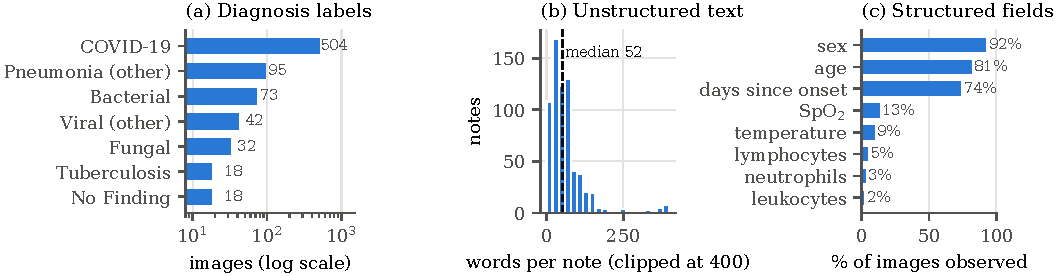
\includegraphics[width=\textwidth]{figures/dataset.pdf}
\caption{Processed dataset. (a) Label counts (log scale). (b) Length of the unstructured
clinical notes (\NotesWith{} of \NImages{} images have one). (c) Fraction of images for which
each structured field is observed; missing values are encoded with learned missing-value
embeddings rather than imputed.}
\label{fig:dataset}
\end{figure*}

%============================================================
\section{Method}
\label{sec:method}
%============================================================
\begin{figure*}[t]
\centering
\resizebox{0.96\textwidth}{!}{% IRENE-MM architecture (TikZ). Included from main.tex.
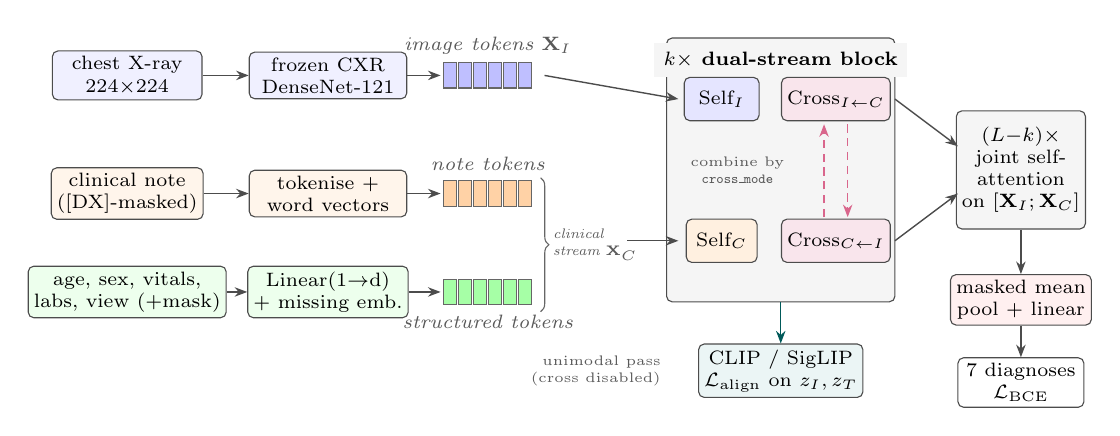
\begin{tikzpicture}[
  font=\scriptsize,
  box/.style={draw=black!70, rounded corners=2pt, minimum height=0.55cm, align=center, inner sep=2pt},
  tok/.style={draw=black!60, minimum width=0.16cm, minimum height=0.32cm, inner sep=0pt},
  arr/.style={-{Stealth[length=1.6mm]}, black!70, line width=0.5pt},
  lab/.style={font=\scriptsize\itshape, text=black!65},
]
% ---------------- inputs
\node[box, fill=blue!6, minimum width=1.9cm] (img) at (0,0) {chest X-ray\\224$\times$224};
\node[box, fill=orange!8, minimum width=1.9cm] (txt) at (0,-1.5) {clinical note\\([DX]-masked)};
\node[box, fill=green!7, minimum width=1.9cm] (tab) at (0,-2.75) {age, sex, vitals,\\labs, view (+mask)};

% ---------------- tokenisers
\node[box, fill=blue!6, minimum width=2.0cm] (cnn) at (2.55,0) {frozen CXR\\DenseNet-121};
\node[box, fill=orange!8, minimum width=2.0cm] (wv) at (2.55,-1.5) {tokenise +\\word vectors};
\node[box, fill=green!7, minimum width=2.0cm] (lin) at (2.55,-2.75) {Linear(1$\to$d)\\+ missing emb.};
\draw[arr] (img) -- (cnn); \draw[arr] (txt) -- (wv); \draw[arr] (tab) -- (lin);

% token strips
\foreach \i in {0,...,5} {\node[tok, fill=blue!25] at (4.1+\i*0.19,0) {};}
\foreach \i in {0,...,5} {\node[tok, fill=orange!35] at (4.1+\i*0.19,-1.5) {};}
\foreach \i in {0,...,5} {\node[tok, fill=green!35] at (4.1+\i*0.19,-2.75) {};}
\node[lab] at (4.58,0.38) {image tokens $\mathbf{X}_I$};
\node[lab] at (4.58,-1.12) {note tokens};
\node[lab] at (4.58,-3.13) {structured tokens};
\draw[arr] (cnn) -- (3.98,0); \draw[arr] (wv) -- (3.98,-1.5); \draw[arr] (lin) -- (3.98,-2.75);
\draw[decorate, decoration={brace, amplitude=3pt, mirror}, black!60] (5.25,-3.0) -- (5.25,-1.3)
  node[midway, right=1pt, lab, align=left, font=\tiny\itshape] {clinical\\stream $\mathbf{X}_C$};

% ---------------- dual-stream blocks
\node[box, fill=black!4, minimum width=2.9cm, minimum height=3.35cm] (dual) at (8.3,-1.2) {};
\node[font=\scriptsize\bfseries, fill=black!4] at (8.3,0.2) {$k\times$ dual-stream block};
\node[box, fill=blue!10, minimum width=0.95cm] (si) at (7.55,-0.3) {Self$_I$};
\node[box, fill=orange!12, minimum width=0.9cm] (sc) at (7.55,-2.1) {Self$_C$};
\node[box, fill=purple!10, minimum width=1.2cm] (ci) at (9.0,-0.3) {Cross$_{I\leftarrow C}$};
\node[box, fill=purple!10, minimum width=1.2cm] (cc) at (9.0,-2.1) {Cross$_{C\leftarrow I}$};
\draw[arr, purple!60, densely dashed] (8.85,-1.8) -- (8.85,-0.62);
\draw[arr, purple!60, densely dashed] (9.15,-0.62) -- (9.15,-1.8);
\node[lab, align=center, font=\tiny] at (7.75,-1.2) {combine by\\\texttt{cross\_mode}};
\draw[arr] (5.3,0) -- (7.0,-0.3);
\draw[arr] (6.35,-2.1) -- (7.0,-2.1);

% ---------------- alignment
\node[box, fill=teal!8, minimum width=1.75cm] (align) at (8.3,-3.75) {CLIP / SigLIP\\$\mathcal{L}_{\text{align}}$ on $z_I, z_T$};
\draw[arr, teal!70!black] (8.3,-2.88) -- (align);
\node[lab, font=\tiny, align=right, anchor=east] at (6.9,-3.75) {unimodal pass\\(cross disabled)};

% ---------------- joint blocks
\node[box, fill=black!4, minimum width=1.6cm, minimum height=1.5cm, align=center] (joint) at (11.35,-1.2) {$(L{-}k)\times$\\joint self-\\attention\\on $[\mathbf{X}_I;\mathbf{X}_C]$};
\draw[arr] (9.75,-0.3) -- (10.55,-0.9); \draw[arr] (9.75,-2.1) -- (10.55,-1.5);
\node[box, fill=red!6, minimum width=1.6cm] (head) at (11.35,-2.85) {masked mean\\pool + linear};
\draw[arr] (joint) -- (head);
\node[box, minimum width=1.6cm] (out) at (11.35,-3.9) {7 diagnoses\\$\mathcal{L}_{\text{BCE}}$};
\draw[arr] (head) -- (out);
\end{tikzpicture}
}
\caption{IRENE-MM. Each modality is tokenised; the image stream $\mathbf{X}_I$ and the clinical
stream $\mathbf{X}_C$ (note + structured tokens) pass through $k$ dual-stream blocks whose
cross-modal exchange is set by \texttt{cross\_mode}, then through $L-k$ joint self-attention blocks.
$k=0$ is early fusion; $k=L$ with no cross-attention is late fusion; IRENE is $k=2$ with
bidirectional attention. The optional alignment loss is computed on \emph{unimodal}
pooled embeddings (a second pass through the dual-stream blocks with cross-attention
disabled), so that the note embedding cannot see the image.}
\label{fig:arch}
\end{figure*}

\paragraph{Tokenisation.} \Cref{fig:arch} shows the architecture. Following the ``hybrid''
tokeniser that IRENE inherits from ViT \citep{dosovitskiy2021vit}, radiographs are encoded by a
DenseNet-121 \citep{huang2017densenet} pretrained on seven public chest X-ray datasets
(\texttt{torchxrayvision} \texttt{densenet121-res224-all} \citep{cohen2022torchxrayvision}),
kept frozen; its $7{\times}7{\times}1024$ feature map is average-pooled to a $4{\times}4$ grid
and linearly projected to $d$-dimensional image tokens with learned position embeddings.
Five views per image (one clean, four randomly cropped, rotated and intensity-jittered) are
cached; training samples a random view per step. Note tokens (at most \MaxTxt{}) are linearly
projected; age and sex use IRENE's scalar embeddings \texttt{Linear(1,$d$)}, and each structured
value $v_j$ with mask $m_j$ becomes $m_j\,W v_j + (1-m_j)\,e^{\text{miss}}_j + p_j$ with a
shared projection $W$, a learned missing embedding and a position embedding.

\paragraph{Dual-stream block.} Let $h_I=\mathrm{LN}(\mathbf{X}_I)$, $h_C=\mathrm{LN}(\mathbf{X}_C)$,
$S_I=\mathrm{Attn}(h_I,h_I)$, $S_C=\mathrm{Attn}(h_C,h_C)$ and the cross terms
$X_{I\leftarrow C}=\mathrm{Attn}(q{=}h_I,kv{=}h_C)$, $X_{C\leftarrow I}=\mathrm{Attn}(q{=}h_C,kv{=}h_I)$,
each with its own projections and key-padding masks. The attention outputs $A_I, A_C$ are
\begin{center}
\small
\begin{tabular}{@{}lll@{}}
\toprule
\texttt{cross\_mode} & $A_I$ & $A_C$ \\
\midrule
\texttt{bi\_avg} (IRENE) & $(S_I+X_{I\leftarrow C})/2$ & $(S_C+X_{C\leftarrow I})/2$\\
\texttt{bi\_cross} (co-attn.) & $X_{I\leftarrow C}$ & $X_{C\leftarrow I}$\\
\texttt{i2t} & $(S_I+X_{I\leftarrow C})/2$ & $S_C$\\
\texttt{t2i} & $S_I$ & $(S_C+X_{C\leftarrow I})/2$\\
\texttt{gated} & $S_I+\tanh(\alpha_I)X_{I\leftarrow C}$ & $S_C+\tanh(\alpha_C)X_{C\leftarrow I}$\\
\texttt{none} & $S_I$ & $S_C$\\
\bottomrule
\end{tabular}
\end{center}
followed by per-stream output projections, residual connections and feed-forward networks.
\texttt{bi\_avg} is IRENE's equation (averaging self- and cross-attention contexts);
\texttt{bi\_cross} corresponds to ViLBERT/LXMERT co-attention \citep{lu2019vilbert,tan2019lxmert};
\texttt{gated} follows Flamingo's zero-initialised tanh gates \citep{alayrac2022flamingo}.

\paragraph{Fusion position.} After $k$ dual-stream blocks the streams are concatenated and
processed by $L-k$ standard pre-LN blocks \citep{vaswani2017attention}. The prediction is a
linear head on the masked mean of all tokens (IRENE also mean-pools). With $k=0$ the model is a
single-stream early-fusion transformer; with $k=L$ and \texttt{none} the streams never interact
and their pooled features are concatenated before the head (late fusion).

\paragraph{Contrastive alignment.} With projection heads $g_I,g_T$ and pooled unimodal
embeddings $z_I, z_T$ (image tokens; note tokens only), the auxiliary loss is either
CLIP/InfoNCE \citep{radford2021clip},
$\mathcal{L}=\tfrac12\big[\mathrm{CE}(\tau S, Y)+\mathrm{CE}(\tau S^\top, Y^\top)\big]$,
or SigLIP \citep{zhai2023siglip},
$\mathcal{L}=-\tfrac1B\sum_{ij}\log\sigma\big(y_{ij}(\tau S_{ij}+b)\big)$, where
$S_{ij}=g_I(z_I^i)^\top g_T(z_T^j)$ on $\ell_2$-normalised vectors and $\tau$ (and $b$) are learned.
Because images of the same patient often share one note, $Y$ marks \emph{all} pairs with
identical notes as positives (multi-positive targets) instead of treating them as negatives.
Following ALBEF \citep{li2021albef} we align before fusing; unlike a naive implementation that
pools the text stream after cross-attention---where the text embedding already contains the
image and retrieval becomes trivial (we observed R@1 $>0.8$ in a pilot)---$z_I,z_T$ come from a
weight-shared pass through the dual-stream blocks with cross-attention switched off.
The total loss is $\mathcal{L}_{\text{BCE}}+\lambda\mathcal{L}_{\text{align}}$.

\paragraph{Missing modalities.} All attention uses key-padding masks, so images without a note
simply have no note tokens. We evaluate every model a second time with the note removed at test
time, and optionally train with \emph{modality dropout} (note removed with probability 0.3).

%============================================================
\section{Experimental setup}
\label{sec:setup}
%============================================================
\paragraph{Model and training.} All variants use $L{=}6$ layers, $d{=}128$, 4 heads and an MLP
width of 256 (\ParamMin--\ParamMax\,M trainable parameters depending on the variant; the frozen DenseNet
is not counted), dropout 0.1. We train with AdamW \citep{loshchilov2019adamw}
(lr $3{\times}10^{-4}$, weight decay 0.05, one-cycle schedule), batch size 32, gradient clipping 1.0,
at most 25 epochs with early stopping on the validation BCE (patience 5), restoring the best
checkpoint. The contrastive projection dimension is 128.

\paragraph{Protocol.} Every configuration is run on the same five folds with \NSeedsMain{} seeds
(main comparison) or 2 seeds (ablations). We report pooled-OOF macro AUROC (mean $\pm$ s.d.\ over
seeds), macro AUPRC, macro F1 and accuracy of the arg-max prediction, a 95\% patient-level
bootstrap interval of the seed-averaged OOF predictions (1{,}000 resamples), and paired
patient-level bootstrap tests between models. Cross-modal retrieval is image$\to$note Recall@$K$
within each test fold (gallery = distinct notes in the fold, $\approx$120), averaged over folds.

\paragraph{Engineering.} The training stack (\texttt{train.py}) uses PyTorch \citep{paszke2019pytorch}
\texttt{DataLoader} workers with pinned memory, persistent workers and prefetching; automatic mixed
precision \citep{micikevicius2018mixed} (fp16 with loss scaling on GPU, bf16 autocast on CPU);
\texttt{DistributedDataParallel} \citep{li2020ddp} launched with \texttt{torchrun}
(NCCL on GPU, Gloo on CPU) with a \texttt{DistributedSampler}; and Weights \& Biases
\citep{biewald2020wandb} logging of every epoch, fold and seed (offline mode; synchronisable with
\texttt{wandb sync}). All experiments in this paper were run on a 2-core CPU machine without a GPU;
\cref{sec:throughput} reports the throughput measurements we could make there.

%============================================================
\section{Results}
\label{sec:results}
%============================================================
\begin{table*}[t]
\centering
\caption{Main comparison (5-fold patient-grouped CV, pooled out-of-fold predictions on all
\NImages{} images; mean$\pm$s.d.\ over 3 seeds, or 2 seeds for the contrastive rows). The 95\% CI is a
patient-level bootstrap of the seed-averaged predictions. F1 and accuracy use the arg-max class.
Parameters are trainable parameters, excluding the frozen DenseNet.}
\label{tab:main}
\small
\begin{tabular}{@{}lcccccc@{}}
\toprule
Model & macro AUROC & 95\% CI & macro AUPRC & macro F1 & Accuracy & Params (M)\\
\midrule
\tabinput{tables/main.tex}
\bottomrule
\end{tabular}
\end{table*}

\subsection{Fusion helps, provided the text branch is competent}
\Cref{tab:main} and \cref{fig:main} summarise the main comparison. Images alone reach
\AUC{img_only} macro AUROC. Structured data alone reaches \AUC{tab_only}, the masked note alone
\AUC{txt_only}, and note plus structured data \AUC{txt_tab_only}. All three fusion paradigms that
use every modality do better: early fusion \AUC{early_fusion}, IRENE mid fusion (k=2)
\AUC{irene_k2} and late fusion \AUC{late_fusion}. A patient-level paired bootstrap
(\cref{tab:sig}) finds IRENE clearly better than image-only (\SIG{img_only}{diff}, 95\% CI
[\SIG{img_only}{lo}, \SIG{img_only}{hi}]). The gain over note + structured is smaller and
borderline (\SIG{txt_tab_only}{diff}, CI [\SIG{txt_tab_only}{lo}, \SIG{txt_tab_only}{hi}],
$p{=}$\SIG{txt_tab_only}{p}). The differences among the three fusion paradigms are within the
bootstrap uncertainty (IRENE vs.\ early: $p{=}$\SIG{early_fusion}{p}; vs.\ late: $p{=}$\SIG{late_fusion}{p}). Early fusion is also the least stable across seeds
(s.d.\ \AUCsd{early_fusion} against \AUCsd{irene_k2} for IRENE).

One engineering detail mattered more than any architectural choice. In a pilot run, the
note branch was built only from static word vectors, truncated to \MaxTxt{} tokens and trained
from scratch on about 500 notes. The note-only model then reached only about 0.58, and fused models
about 0.71--0.74. A single \emph{document token} fixes this: a TF-IDF$\to$SVD embedding
of the entire note, fitted inside each training fold, plays the role of IRENE's BERT sentence
features. With it and class-balanced BCE, the note-only model rises to \AUC{txt_only} and the
fused models to about 0.78--0.79. \Cref{tab:ablation} isolates the document token
(\AUC{irene_k2_nodoc} without it versus \AUC{irene_k2} with it).

\begin{figure}[t]
\centering
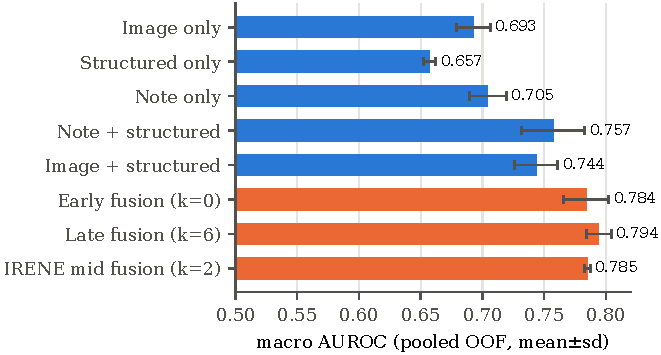
\includegraphics[width=\columnwidth]{figures/main_results.pdf}
\caption{Macro AUROC by input and fusion paradigm. Blue: one or two modalities.
Orange: all three modalities fused. Error bars: s.d.\ over 3 seeds.}
\label{fig:main}
\end{figure}

\begin{table}[t]
\centering
\caption{Patient-level paired bootstrap (1{,}000 resamples) of the macro-AUROC difference
between IRENE (k=2) and other models, using seed-averaged out-of-fold predictions.}
\label{tab:sig}
\small
\setlength{\tabcolsep}{4pt}
\begin{tabular}{@{}lccc@{}}
\toprule
IRENE (k=2) & $\Delta$AUROC & 95\% CI & $p$\\
\midrule
\tabinput{tables/significance.tex}
\bottomrule
\end{tabular}
\end{table}

\begin{table*}[t]
\centering
\caption{Ablations (pooled-OOF macro AUROC and AUPRC, mean$\pm$s.d.\ over seeds). ``No note''
re-evaluates the same model with the note removed at test time. R@5 is image$\to$note retrieval
in \% (chance $\approx$4\%).}
\label{tab:ablation}
\small
\begin{tabular}{@{}lccccc@{}}
\toprule
Variant & macro AUROC & macro AUPRC & AUROC, no note & R@5 & seeds\\
\midrule
\tabinput{tables/ablation.tex}
\bottomrule
\end{tabular}
\end{table*}

\subsection{Where to fuse}
\Cref{fig:fusion} varies the number $k$ of dual-stream blocks with IRENE's bidirectional
attention, keeping depth fixed at $L{=}6$. One or two blocks of cross-modal attention followed
by joint self-attention (k=1: \AUC{irene_k1}; k=2: \AUC{irene_k2}) perform as well as early
fusion. Accuracy then falls as fusion is delayed with cross-attention active (k=3: \AUC{irene_k3};
k=4: \AUC{irene_k4}). It collapses when all six blocks are bidirectional (k=6: \AUC{irene_k6}).
Yet the same depth \emph{without} cross-attention, i.e.\ plain late fusion, is the best model
(\AUC{late_fusion}). The pattern suggests that, on a few hundred training patients, the
extra cross-attention parameters (\cref{tab:main}) and the repeated mixing of a noisy note
into the image stream cause overfitting rather than useful alignment. IRENE's choice of shallow
cross-modal attention followed by joint layers is a sensible point on this curve. The
original paper, with about 10$\times$ more patients, did not report this sweep.

\begin{figure*}[t]
\centering
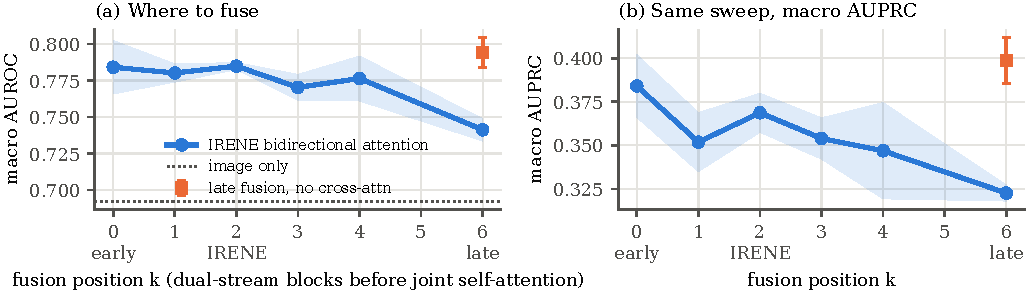
\includegraphics[width=\textwidth]{figures/fusion_position.pdf}
\caption{Fusion position. $k$ dual-stream IRENE blocks are followed by $6-k$ joint blocks;
$k{=}0$ is early fusion. Orange square: $k{=}6$ without cross-attention (late fusion). Dotted
line: image only. Shaded bands and error bars: $\pm$1 s.d.\ over seeds.}
\label{fig:fusion}
\end{figure*}

\subsection{How the streams attend to each other}
\Cref{fig:attn} fixes $k{=}2$ and changes only the combination rule. IRENE's average of self-
and cross-attention (\AUC{irene_k2}) matches the unidirectional variants (image$\to$text
\AUC{attn_i2t}, text$\to$image \AUC{attn_t2i}) and the no-exchange control (\AUC{attn_none}).
It clearly beats ViLBERT-style co-attention, which drops self-attention in the dual-stream
blocks (\AUC{attn_bi_cross}). Flamingo-style tanh gates (\AUC{attn_gated}) are the least
stable across seeds (s.d.\ \AUCsd{attn_gated}). The practical conclusion is that each stream
must keep its intra-modal self-attention. Cross-attention in the first blocks is not harmful,
but at this data scale the joint self-attention layers can recover most of what it provides.
\Cref{fig:attn}b repeats the evaluation with the note removed. All variants fall to 0.58--0.61,
which shows that the models rely heavily on the note whatever the attention structure.

\begin{figure*}[t]
\centering
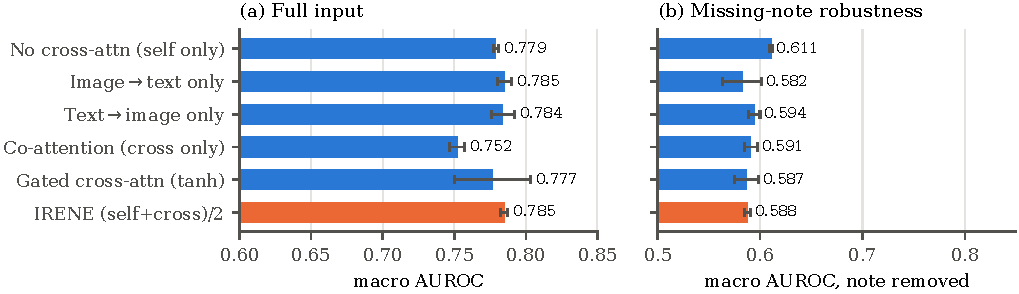
\includegraphics[width=\textwidth]{figures/attention_structure.pdf}
\caption{Attention structure inside the $k{=}2$ dual-stream blocks. (a) Full input.
(b) The same trained models evaluated with the clinical note removed.}
\label{fig:attn}
\end{figure*}

\subsection{Image--text contrastive learning}
\Cref{fig:contrastive} adds a CLIP or SigLIP loss on unimodal pooled embeddings. For IRENE
(k=2), both objectives \emph{lower} diagnostic AUROC, and more so as $\lambda$ grows (CLIP:
\AUC{clip_l0.1}, \AUC{clip_l0.5}, \AUC{clip_l1.0}; SigLIP: \AUC{siglip_l0.1}, \AUC{siglip_l0.5},
\AUC{siglip_l1.0}). SigLIP degrades more gracefully than CLIP. Retrieval is above chance but
modest (R@5 \RFIVE{clip_l0.5}\% for CLIP at $\lambda{=}0.5$, against about 4\% for chance). The
picture changes for late fusion. The two encoders are then separate, so the model is a CLIP-style
dual encoder with a classification head. Alignment leaves AUROC unchanged (\AUC{late_clip_l0.5}
against \AUC{late_fusion}) and gives the best retrieval (R@5 \RFIVE{late_clip_l0.5}\%). In the
early-fusion model the aligned embeddings sit at the token level, and alignment reaches
\AUC{early_clip_l0.5}.

Two properties of this dataset explain the weak benefit. First, there are only about 500
training pairs per fold, and many images of the same patient share one note, so the effective
number of distinct pairs is small. Second, the notes describe history and radiographic findings
in heterogeneous styles, with no one-to-one correspondence to the image. Contrastive
pre-training works at the scale of hundreds of thousands to millions of report pairs
\citep{zhang2022convirt,you2023cxrclip,zhang2023biomedclip}. As an auxiliary loss on hundreds
of pairs, it competes with the supervised objective for the shared parameters in the
dual-stream blocks, which is why it hurts mid fusion but not a dual encoder.

\begin{figure*}[t]
\centering
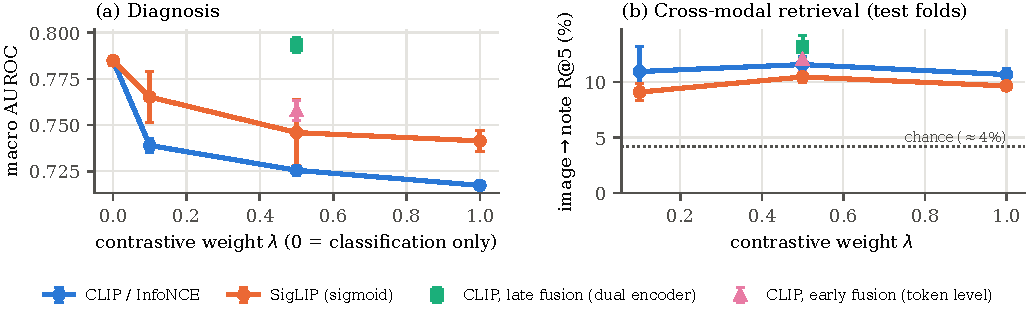
\includegraphics[width=\textwidth]{figures/contrastive.pdf}
\caption{Contrastive alignment. (a) Diagnostic macro AUROC as a function of the alignment
weight $\lambda$ ($\lambda{=}0$ is IRENE without alignment). (b) Image$\to$note Recall@5 on
the test folds.}
\label{fig:contrastive}
\end{figure*}

\subsection{Per-class behaviour}
\Cref{fig:perclass,fig:roc} break results down by class. Compared with the image-only model, fusion gains the most for
COVID-19 (IRENE \PC{irene_k2}{0} vs.\ \PC{img_only}{0}), bacterial pneumonia
(\PC{irene_k2}{2} vs.\ \PC{img_only}{2}) and unspecified pneumonia (\PC{irene_k2}{4} vs.\
\PC{img_only}{4}). The note-based models are strong on exactly these classes (note + structured:
\PC{txt_tab_only}{0}, \PC{txt_tab_only}{2}, \PC{txt_tab_only}{4}). The image contributes more for
fungal pneumonia (image-only \PC{img_only}{3} vs.\ note + structured \PC{txt_tab_only}{3}), where
fusion combines both (\PC{irene_k2}{3}). Tuberculosis and no finding (18 images each) remain the
hardest and noisiest classes for every model.

\begin{figure}[t]
\centering
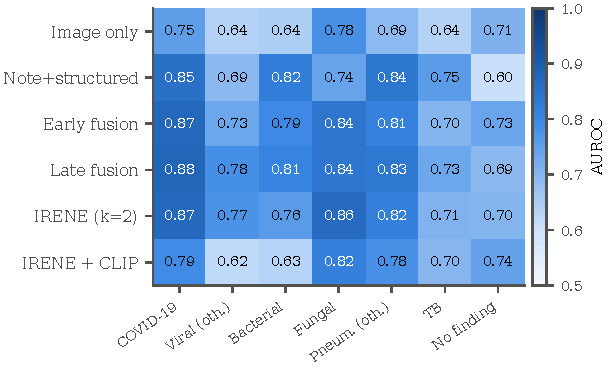
\includegraphics[width=\columnwidth]{figures/per_class.pdf}
\caption{Per-class AUROC (pooled OOF, mean over seeds).}
\label{fig:perclass}
\end{figure}

\begin{figure*}[t]
\centering
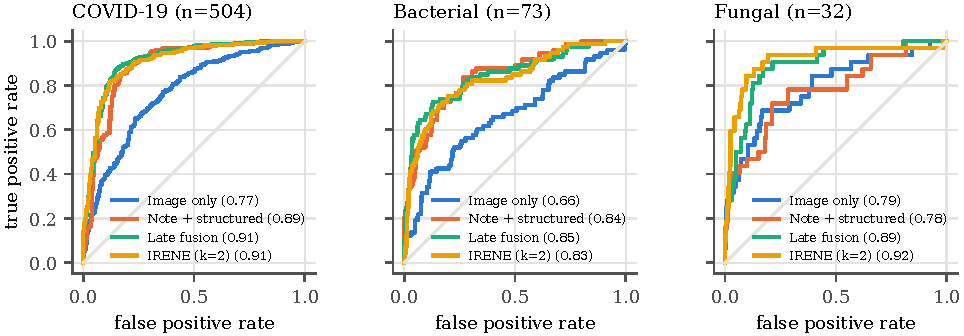
\includegraphics[width=\textwidth]{figures/roc.pdf}
\caption{Pooled out-of-fold ROC curves (seed-averaged predictions) for three classes;
AUROC in the legend.}
\label{fig:roc}
\end{figure*}

\subsection{Label leakage and dataset confounding}
\label{sec:leak}
\begin{table}[t]
\centering
\caption{Shortcut probes. Macro AUROC on all \NImages{} images and on the \NMixed{} images from the
two case repositories that contain \emph{both} COVID-19 and non-COVID cases (Radiopaedia,
Eurorad), where the source cannot identify the label. Logistic regressions use the same folds.}
\label{tab:reference}
\small
\setlength{\tabcolsep}{4pt}
\begin{tabular}{@{}lcc@{}}
\toprule
Model & all images & mixed-source subset\\
\midrule
\tabinput{tables/reference.tex}
\bottomrule
\end{tabular}
\end{table}

\paragraph{Diagnosis terms in notes.} \PctMasked\% of the notes name the diagnosis or the
pathogen. Leaving these terms unmasked raises note + structured from \AUC{txt_tab_only} to
\AUC{txt_tab_only_rawtext} and IRENE from \AUC{irene_k2} to \AUC{irene_k2_rawtext}
(\cref{fig:robust}a). The gain is smaller than one might expect, because the remaining text is
itself highly predictive. A TF-IDF logistic regression on the \emph{masked} notes reaches
\CL{tfidf_masked}, almost as high as on raw notes (\CL{tfidf_raw}), and above every transformer
in this study (\cref{tab:reference}). Masking is still necessary for a fair evaluation, but it is
far from sufficient.

\paragraph{Source confounding.} Public COVID-19 collections gather cases from sources that
differ systematically in their label mix. Some are almost entirely COVID-19 (the SIRM archive,
GitHub-hosted hospital releases, NEJM case reports), while others are mostly non-COVID
(Eurorad). A logistic regression that sees \emph{only} the host of the source URL reaches
\CL{source_only} macro AUROC, on par with the fusion transformers. The notes and the view
(\CL{view_only}) carry this signal implicitly through writing style, translation artefacts
and acquisition protocol. As a de-confounded check, we recompute every metric on the \NMixed{}
images from Radiopaedia and Eurorad, the two repositories that host both COVID-19 and
non-COVID cases. There the source-only probe falls to chance (\CL{source_only@mixed}). The fused models
lose about 6 points and the image-only model about 3, but the ranking is preserved (\cref{tab:reference}). Late fusion
(\MIX{late_fusion}), early fusion (\MIX{early_fusion}) and IRENE (\MIX{irene_k2}) remain above
note + structured (\MIX{txt_tab_only}) and image-only (\MIX{img_only}). The TF-IDF note model is
still the strongest (\CL{tfidf_masked@mixed}). This agrees with the radiograph shortcuts reported
by DeGrave et al.\ \citep{degrave2021shortcuts} and argues for reporting a de-confounded subset
alongside headline numbers on public COVID-19 data.

\begin{figure*}[t]
\centering
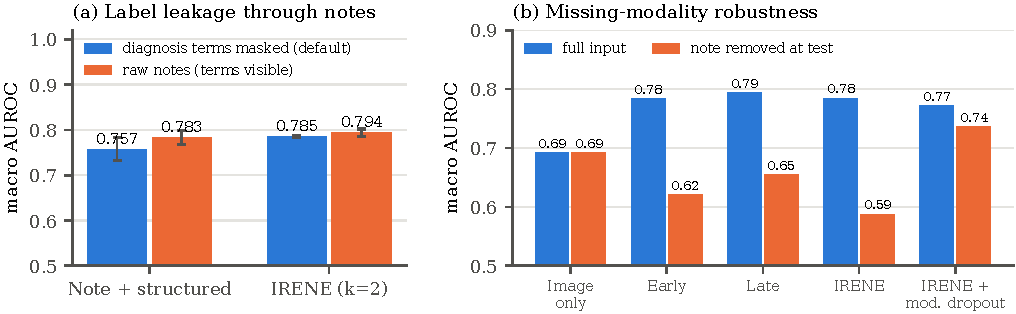
\includegraphics[width=\textwidth]{figures/robustness.pdf}
\caption{(a) Effect of masking diagnosis and pathogen names in the notes (2 seeds for the
raw-note runs). (b) Macro AUROC with the full input and with the note removed at test time.
Modality dropout ($p{=}0.3$) during training closes most of the gap.}
\label{fig:robust}
\end{figure*}

\paragraph{Missing notes.} Deployed systems will not always have a note. When it is removed at
test time, IRENE falls from \AUC{irene_k2} to \NT{irene_k2}, well below the image-only model
(\AUC{img_only}). Early and late fusion degrade less (\NT{early_fusion} and \NT{late_fusion};
\cref{fig:robust}b). The fused models have learned to rely on the note and do not fall back on
the image features. This matches the fragility reported by Ma et al.\ \citep{ma2022missing}.
Training with modality dropout ($p{=}0.3$) raises the no-note AUROC to \NT{irene_k2_moddrop},
close to the image + structured model (\AUC{img_tab}), at a small cost with full input
(\AUC{irene_k2_moddrop}). For a clinical deployment where the note is not always available,
this trade-off is clearly worthwhile.


\subsection{Throughput of the training stack}
\label{sec:throughput}
\begin{figure*}[t]
\centering
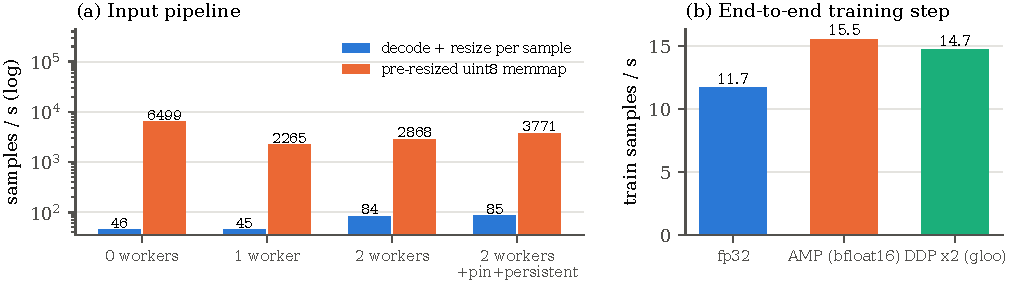
\includegraphics[width=\textwidth]{figures/throughput.pdf}
\caption{Throughput on the 2-core CPU machine used for all experiments. (a) Input pipeline:
decoding and resizing the original radiographs per sample, versus a pre-resized uint8
memory-mapped cache, for several \texttt{DataLoader} settings. (b) One end-to-end training step
of pixel-input IRENE-MM (batch 16), in fp32, with bf16 autocast, and with DDP over 2 Gloo
processes (1 thread each).}
\label{fig:throughput}
\end{figure*}

\Cref{fig:throughput} reports the engineering measurements we could make without a GPU.
Many source radiographs are large JPEG/PNG files, and decoding and resizing them for every
sample limits the input pipeline to \TpDecodeZero{} samples/s in the main process. Two worker
processes help ($\times$\TpWorkerSpeedup{}, \TpDecodeBest{} samples/s). Pre-resizing once into a
memory-mapped uint8 array takes \TpCacheSec{}\,s and raises throughput to \TpMmapBest{}
samples/s ($\times$\TpSpeedup{}). With so little per-sample work on 2 cores, worker processes
then \emph{reduce} throughput because of inter-process transfer. The right
\texttt{num\_workers} depends on the per-sample cost, and should be measured rather than set
by habit. Persistent workers avoid re-forking at every epoch and help consistently when
workers are used. For the model, bf16 autocast raises end-to-end training throughput from
\TpFp{} to \TpAmp{} samples/s on this CPU. DDP with two single-threaded Gloo ranks reaches
\TpDDP{} samples/s, against \TpFp{} for one process with two threads. The same \texttt{train.py}
runs unchanged with NCCL and fp16 loss scaling on GPUs, but we could not measure GPU
utilisation here and make no claim about it.


%============================================================
\section{Discussion}
%============================================================
\paragraph{What matters for IRENE-style fusion at small scale.}
Three findings are consistent across metrics and seeds.
(1)~\emph{Fusion helps, and the text representation decides by how much.} Adding the note
and structured data to the image raises macro AUROC by about 0.09--0.10. However, a weak note
encoder (static word vectors alone) wiped out most of this gain. A document-level token
recovered it.
(2)~\emph{Keep intra-modal self-attention, and limit cross-attention to early layers.}
IRENE's (self+cross)/2 blocks followed by joint self-attention are on par with early and
late fusion. Cross-attention without self-attention, or cross-attention at every layer, is
clearly worse. On a few hundred patients, extra cross-modal capacity causes overfitting.
(3)~\emph{Contrastive alignment is not free.} As an auxiliary loss on hundreds of pairs,
CLIP and SigLIP hurt a mid-fusion model and are neutral for a dual encoder. The benefit reported
for medical vision--language models comes from large-scale pre-training, which our setting
lacks. A natural next step is to initialise the two streams from a publicly released
radiograph--report encoder (e.g.\ BiomedCLIP or CXR-CLIP) instead of learning the alignment
on the target data.

\paragraph{What the headline numbers hide.} The dataset is public, multimodal and, with IRENE's
input types, a natural testbed. It is also strongly confounded by source. A source-only probe
matches the fusion transformers, and a linear bag-of-words model on the masked notes beats all
of them. The de-confounded subset preserves the ranking of the fusion strategies, which supports
the architectural conclusions. The absolute numbers, however, should not be read as clinical
diagnostic accuracy.

%============================================================
\section{Limitations}
\label{sec:limits}
%============================================================
\begin{itemize}
\item \textbf{Scale.} \NImages{} images from \NPatients{} patients, and three or fewer positives
per test fold for some classes. We pool out-of-fold predictions and report bootstrap intervals.
Many ablation differences are nevertheless within noise, and the ablations use 2 seeds.
\item \textbf{Compute.} No GPU was available. The model is a narrow IRENE ($d{=}128$, 6 layers,
16 image tokens from a frozen CNN) rather than the original ViT-B/16 initialised from ImageNet
weights, and the text encoder is not a clinical BERT. The recipe was revised once, after a full
cross-validation pilot showed that the note branch was the bottleneck (it added the document token
and class-balanced loss). This single round of development used out-of-fold results, so a fresh
external test set would be needed for an unbiased estimate.
\item \textbf{Data.} The labels come from publication metadata, the notes are written by case
authors rather than being contemporaneous EHR text, and the source confounding described in
\cref{sec:leak} limits clinical interpretation. The engineering code supports large sharded
image--text corpora and multi-GPU training, but this study did not exercise that scale.
\end{itemize}

%============================================================
\section{Conclusion}
%============================================================
We provide an open, end-to-end re-implementation of the IRENE multimodal transformer on
public data. It includes a documented image--text--structured pipeline, a modern PyTorch
training stack, a single model that covers early, mid and late fusion, six attention structures
and two contrastive objectives, and a controlled study with patient-grouped cross-validation.
The results support IRENE's core design: shallow bidirectional attention that retains
self-attention, followed by joint layers. They also show that a competent text representation,
robustness to missing notes and awareness of dataset confounding matter more than the
particular choice of fusion operator.



{\small
\bibliographystyle{unsrtnat}
\bibliography{refs}
}

\appendix
\section{Reproducibility details}
\label{app:repro}

\paragraph{Code.} Everything is in the repository:
\texttt{data/prepare.py} (cohort, labels, text cleaning, masking, structured features, folds),
\texttt{data/features.py} (frozen CXR DenseNet tokens with cached augmentations; word-vector note tokens),
\texttt{models/irene\_mm.py} (IRENE-MM), \texttt{train.py} (CV training with AMP/DDP/W\&B),
\texttt{scripts/run\_experiments.py} (the full grid),
\texttt{scripts/classical\_baselines.py}, \texttt{scripts/benchmark\_throughput.py} and
\texttt{scripts/make\_figures.py} (all figures, tables and every number quoted in the text,
emitted as LaTeX macros). The original IRENE files in \texttt{models/} and \texttt{irene.py} are
kept, with the deprecated \texttt{apex} AMP replaced by \texttt{torch.autocast}.

\paragraph{Pretrained components.} Image: \texttt{torchxrayvision} DenseNet-121
\texttt{densenet121-res224-all}, trained on NIH ChestX-ray14, CheXpert, MIMIC-CXR, PadChest,
RSNA Pneumonia (Kaggle), Google and OpenI radiographs \citep{cohen2022torchxrayvision}; none of these
is the evaluation dataset, but overlap of individual source images cannot be excluded.
Text: spaCy \texttt{en\_core\_web\_md} 300-d vectors (20k keys). No component was pretrained on the
evaluation notes.

\paragraph{Hyper-parameters.} $L{=}6$, $d{=}128$, 4 heads, MLP 256, dropout and attention dropout
0.1, image grid $4{\times}4$ (16 tokens), at most \MaxTxt{} word tokens plus one 128-d TF-IDF/SVD
document token fitted inside each training fold, 11 structured tokens plus age and sex tokens,
AdamW (lr $3{\times}10^{-4}$, wd 0.05), one-cycle schedule with 10\% warm-up, batch 32,
$\le$25 epochs, early stopping on validation BCE with patience 5, positive-class weights
$\sqrt{n_{\text{neg}}/n_{\text{pos}}}$ in the BCE, gradient clipping 1.0, CLIP temperature
initialised at 0.07, SigLIP $t{=}10$, $b{=}{-}10$ \citep{zhai2023siglip}. No per-configuration tuning
was done. However, the recipe was revised once: a first full cross-validation pilot of the eight
main configurations (kept in \texttt{results/runs\_v0\_pilot/}) showed that the note branch was
the bottleneck, and we then added the document token and the class-balanced loss and reran
everything. Because that decision was informed by out-of-fold results, the reported estimates
are slightly optimistic in the usual ``one round of model development'' sense
(\cref{sec:limits}).

\paragraph{Compute.} All \NRuns{} configurations (\NFoldRuns{} fold-level trainings) ran in
\CPUHours{} CPU-hours on a 2-core virtual machine without a GPU.

\end{document}
